%\section{Arquiteturas de WebApps?}
%%-------------------------------------------------------------------------------------- Início
\begin{frame}[allowframebreaks, fragile,t]{Arquiteturas de Aplicações Web}
  \begin{itemize}
    \item As aplicações \alert{web modernas} envolvem uma quantidade significativa de \alert{complexidade}.
    \begin{itemize}
      \item especialmente no lado do servidor.
    \end{itemize}
    \item Uma típica aplicação web envolve \alert{inúmeros protocolos}, \alert{linguagens de programação} e 
      \alert{tecnologias} que compõem a pilha de tecnologia web. 
    \item Desenvolver, manter e ampliar uma aplicação web complexa é \alert{difícil}.
    \begin{itemize}
      \item mas, construindo-o usando uma \alert{base de princípios de sólidos de projeto} pode-se simplificar 
      cada uma dessas tarefas. 
    \end{itemize}
    \item Engenheiros de software usam \alert{abstrações} para lidar com este tipo de complexidade.
    \begin{itemize}
      \item \textit{Design patterns} fornecem abstrações úteis para sistemas orientados a objetos.
    \end{itemize} 
  \end{itemize}
\end{frame}
%%-------------------------------------------------------------------------------------- Início
\begin{frame}[allowframebreaks, fragile,t]{Design Patterns}
  \begin{exampleblock}{Definição (Design Patterns)}
    Um padrão de projeto é uma descrição da \alert{colaboração de objetos} que interagem para resolver 
    um problema de software em geral dentro de um contexto particular.
  \end{exampleblock}
  \begin{itemize}
    \item Um design pattern é um \alert{modelo abstrato} que pode ser aplicado recorrentemente.
    \item A idéia é aplicar padrões de projeto, a fim de \alert{resolver problemas específicos} que ocorrem 
      durante a construção de sistemas reais.
    \item Os padrões de projeto fornecem uma maneira de \alert{comunicar} as soluções em um projeto, ou seja, 
      é a terminologia que engenheiros de software usam para falar sobre projetos.
  \end{itemize}
\end{frame}
%%-------------------------------------------------------------------------------------- Início
\begin{frame}[allowframebreaks, fragile,t]{Modelo Cliente-Servidor}
	\begin{itemize}
		\item A arquitetura \alert{cliente-servidor} é a arquitetura mais básica para descrever a cooperação
		entre os componentes de uma aplicação web.
		\item A arquitetura cliente-servidor pode ser subdividia em:
		\begin{itemize}
			\item \alert{servidor} que "escuta" por requisições e fornece os serviços ou recursos de acordo com 
			cada  uma.
			\item \alert{cliente} que estabelece a conexão com o servidor para requisitar serviços ou recursos.
		\end{itemize}
		\item Existe um protocolo \alert{request/response} associado com qualquer arquitetura cliente-servidor.
	\end{itemize}
	\begin{figure}[h!]
		\centering
		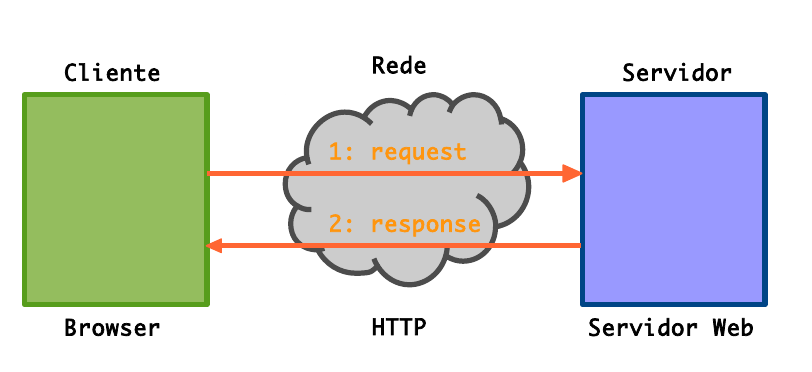
\includegraphics[width=0.90\textwidth]{imagens/cliente-servidor-1.png}
		\caption{Arquitetura cliente servidor.}
	\end{figure} 
	
\framebreak
  \begin{itemize}
    \item É sem dúvida é o padrão de projeto de arquitetura mais conhecido
    \item O ponto chave de uma arquitetura cliente-servidor é \alert{distribuir} os componentes de uma 
      aplicação entre o cliente o servidor de alguma forma. 
    \begin{itemize}
        \item o servidor realiza as tarefas, consultas e transações
        \item o cliente fica com uma responsabilidade menor: a de receber informações
    \end{itemize} 
    \item A fim de construir aplicações web complexas, vários design patterns ajudam a \alert{organizar} como peças 
      são dispostas dentro da arquitetura cliente-servidor.
  \end{itemize}
\end{frame}
%%-------------------------------------------------------------------------------------- Início
\begin{frame}[allowframebreaks, fragile,t]{Arquitetura N-Tier}
  \begin{exampleblock}{Definição (Arquitetura N-Tier)}
    A arquitetura n-tier é um \textit{design pattern} muito útil que estrutura o modelo cliente-servidor.
  \end{exampleblock}
  \begin{itemize}
    \item Este padrão de projeto é baseado no conceito de \alert{quebrar} um sistema em partes diferentes ou 
      camadas que podem ser separados fisicamente:
    \begin{itemize}
      \item cada camada é responsável por fornecer uma \alert{funcionalidade específica} ou coesa. 
      \item uma camada apenas interage com as \alert{camadas adjacentes} a ela por meio de uma 
	\alert{estrutura} bem definida por meio de \alert{interfaces}.
    \end{itemize}
  \end{itemize}
  \begin{exampleblock}{Exemplos (Arquitetura 2-Tier)}
    \begin{itemize}
      \item Servidores de impressão
      \item Aplicações web antigas:
      \begin{itemize}
        \item Interface com o usuário (navegador) residia no cliente (thin). 
        \item Servidor fornecia as páginas estáticas (HTML). 
        \item Interface entre os dois via \textit{Hypertext Transfer Protocol} (HTTP).
      \end{itemize}
    \end{itemize}
  \end{exampleblock}
  \begin{itemize}
    \item Camadas \alert{adicionais} aparecem quando a \alert{funcionalidade} do aplicativo é ainda 
      \alert{mais dividida}.
    \item Quais são as vantagens de um tal projeto? 
    \begin{itemize}
      \item A abstração fornece um meio para \alert{gerenciar} a complexidade. 
      \item Camadas podem ser atualizados ou substituídos de forma \alert{independente} 
	a medida que os requisitos ou tecnologia.
      \begin{itemize}
       \item  a nova só precisa usar as \alert{mesmas interfaces} que a antiga utilizada. 
      \end{itemize}
      \item Ele fornece um \alert{equilíbrio} entre inovação e padronização. 
      \item Sistemas tendem a ser muito mais \alert{fáceis} de construir, manter e atualizar.
    \end{itemize}
  \end{itemize}

\end{frame}
%%-------------------------------------------------------------------------------------- Início
\begin{frame}[allowframebreaks, fragile,t]{Arquitetura 3-Tiers}
  \begin{itemize}
    \item Uma das mais comuns é a arquitetura em 3 camadas: 
    \begin{itemize}
      \item Apresentação
      \begin{itemize}
       \item a interface com o usuário. 
      \end{itemize}     
      \item Aplicação (lógica)
      \begin{itemize}
	\item recupera modifica e$/$ou exclui dados na camada de dados, e envia os resultados do processamento
	para a camada de apresentação. 
      \end{itemize}
      \item Camada de dados
      \begin{itemize}
       \item a fonte dos dados associados ao aplicativo.
      \end{itemize}
    \end{itemize}
 
    \item As aplicações web modernas frequentemente são construídas \alert{utilizando} uma arquitetura em 3 camadas: 
    \begin{itemize}
      \item Apresentação
      \begin{itemize}
	\item o navegador web do usuário. 
      \end{itemize}

      \item Aplicação (lógica) 
      \begin{itemize}     
	\item o servidor web e lógica associada com \alert{geração} de conteúdo web dinâmico.
	\item por exemplo, a coleta e formatação do resultados de uma pesquisa. 
      \end{itemize}
      
      \item Camada de dados
      \begin{itemize}    
	\item um banco de dados.
      \end{itemize}
      
    \end{itemize}
    
  \end{itemize}
\end{frame}
%%-------------------------------------------------------------------------------------- Início
%\begin{frame}[allowframebreaks, fragile,t]{Arquitetura 6-Tiers para Aplicações Web }
%  \begin{itemize}
%    \item A camada de aplicação é frequentemente subdividida em dois níveis:
%    \begin{itemize} 
%      \item Camada de lógica de negócios
%      \begin{itemize}
%	\item modelos os \alert{objetos de negócios} associados ao aplicativo, por exemplo, contas, estoques, etc.
%	\item captura as regras de negócio associadas a esses objetos.     
%       \end{itemize}      
%      \item Camada de acesso a dados
%      \begin{itemize}
%	\item responsável por acessar os dados e passá-los para a camada de lógica de negócios.
%	\item por exemplo, saldos de contas, transações, etc.
%      \end{itemize}
%    \end{itemize}
%    \item A camada de apresentação é muitas vezes subdividida em dois níveis: 
%    \begin{itemize}
%      \item Camada de clientes
%      \begin{itemize}
%	\item os componentes da interface do usuário do lado do cliente.
%      \end{itemize}
%      
%      \item Apresentação camada de lógica
%      \begin{itemize}
%       \item scripts do lado do servidor para a geração de páginas web. 
%      \end{itemize}
%
%    \end{itemize}
%    \item Finalmente, o servidor web é muitas vezes separados em sua própria camada da Web e o
%    servidor de banco de dados na sua camada de dados.
%  \end{itemize}
%  
%  \begin{figure}[h!]
%    \centering
%    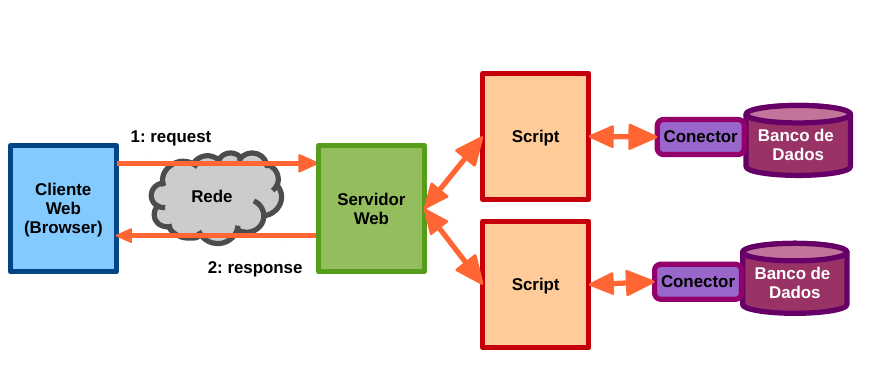
\includegraphics[width=0.95\textwidth]{imagens/cliente-servidor-2.png}
%    \caption{Arquitetura em 6 Camadas.}
%  \end{figure}
%  
%\end{frame}
%%%-------------------------------------------------------------------------------------- Início